\documentclass[10pt, a4paper]{article}
\usepackage[paper=a4paper, left=1.5cm, right=1.5cm, bottom=1.5cm, top=1.5cm]{geometry}
\usepackage[utf8]{inputenc}
\usepackage[spanish]{babel}
\usepackage[autor]{caratula}
\usepackage[pdfencoding=auto, colorlinks=true, linkcolor=blue]{hyperref}
\usepackage[boxed, longend]{algorithm2e}
\usepackage{amsmath}
\usepackage{graphicx}

\SetKwComment{Comment}{}{}
\SetKwInput{Pre}{Pre}
\SetKwInput{Post}{Post}

\begin{document}

% CARATULA
\materia{Algoritmos y Estructuras de Datos III}
\submateria{Primer Cuatrimestre de 2017}
\fecha{\today}
\titulo{Trabajo Práctico 1}

\integrante{Szperling, Sebastián Ariel}{763/15}{sszperling@dc.uba.ar}

\maketitle

% compilar 2 veces para actualizar las referencias
\tableofcontents

\pagebreak
\section{Descripción del problema}

	\subsection{Descripción general}
	El problema propuesto pide que se encuentre la menor cantidad "elementos sin pintar" posibles para una lista de números enteros siguiendo el siguiente criterio:
	
	\begin{itemize}
		\item Todos los elementos pueden solo estar pintados de azul, de rojo, o estar sin pintar (mutuamente exclusivos).
		\item Todos los elementos pintados de rojo deben estar en orden \textit{estrictamente creciente}.
		\item Todos los elementos pintados de azul deben estar en orden \textit{estrictamente decreciente}.
	\end{itemize}

	El problema, para una lista dada de números, se considera que tiene una resolución \textbf{óptima} si existe una manera de pintar todos los elementos de dicha lista ya sea de rojo o de azul, es decir, no queda ningún elemento sin pintar.

	\subsection{Ejemplos provistos por la cátedra}
	
	Para estos ejemplos, se denotará debajo de cada número con una letra si el mismo se pinta de \textbf{R}ojo, \textbf{A}zul o \textbf{N}o pintado.

	\begin{enumerate}
		\item Ejemplo con solución óptima

		\begin{tabular}{ c c c c c c c c }
			0 & 7 & 1 & 2 & 2 & 1 & 5 & 0 \\
			R & A & R & R & A & A & R & A \\
		\end{tabular}

		Resultado: 0 (óptima)

		En este ejemplo se pueden encontrar subsecuencias que cumplan los criterios mencionados: una de elementos rojos (0 1 2 5) y otra de elementos azules (7 2 1 0).

		\item Ejemplo sin solución óptima

		\begin{tabular}{ c c c c c c c c c c c c }
			3 & 11 & 0 & 1 & 3 & 5 & 2 & 4 & 1 & 0 & 9 & 3 \\
			N & A & R & R & R & A & A & R & A & A & R & N \\
		\end{tabular}

		Resultado: 2

		En este ejemplo, no existe un par de subsecuencias disjuntas que satisfagan todos los criterios, por lo que el primer y el último 3 son ignorados para maximizar la cantidad de elementos pintados.
	\end{enumerate}

	\subsection{Otros ejemplos}

	\begin{enumerate}
		\item Ejemplo con único número

		\begin{tabular}{ c c c c c c c c }
			0 & 0 & 0 & 0 & 0 & 0 & 0 & ... \\
			R & A & N & N & N & N & N & ... \\
		\end{tabular}

		Resultado: longitud de la lista - 2

		Para cualquier longitud de lista, si la misma solo contiene elementos idénticos, solo pueden pintarse 2 elementos (ya que los rojos y los azules deben ser \underline{estrictamente} crecientes y decrecientes respectivamente).
	\end{enumerate}


\pagebreak
\section{Resolución por \textit{Backtracking}}
	\subsection{Descripción del algorítmo}

	La solución por Bactracking emplea recursividad en cada paso, y recorre el espacio de soluciones como si el mismo fuese un arbol en preorden.

	A continuación se propone un algoritmo para las llamadas recursivas. Para el caso inicial, se toma $Indice = 0$ y $Res = 0$.

	\begin{algorithm}[H]
		\KwData{Lista, la lista de números a pintar}

		\KwData{UltRojo, el valor del úlitmo rojo que pintamos (si existe)}

		\KwData{UltAzul, el valor del úlitmo azul que pintamos (si existe)}

		\KwData{Indice, la posición que estamos mirando ahora}

		\KwData{Res, la cantidad de elementos no pintados hasta ahora}

		\eIf{Indice == $|Lista|$}{
			Llegamos al final de la lista, no hacer nada
		}{
			Calcular el mejor resultado sin pintar

			Llamada Recursiva: \{Lista, UltRojo, UltAzul, Indice+1, Res+1\}

			Guardar ese resultado como Res

			\If{no existe UltRojo \textbf{or} UltRojo $<$ Lista[Indice]}{
				Calcular el mejor resultado pintando de Rojo

				Llamada Recursiva: \{Lista, Lista[Indice], UltAzul, Indice+1, Res\}

				Si ese resultado es menor que Res, guardarlo como Res
			}
			\If{no existe UltAzul \textbf{or} UltAzul $>$ Lista[Indice]}{
				Calcular el mejor resultado pintando de Azul

				Llamada Recursiva: \{Lista, UltRojo, Lista[Indice], Indice+1, Res\}

				Si ese resultado es menor que Res, guardarlo como Res
			}
		}

		\KwResult{Res, la menor de todas las sub-soluciones}
	\end{algorithm}

	Cabe destacar que el orden en que se calculan los posibles resultados no es relevante, en tanto se conserve el menor de todos.

	En la implementación propuesta, UltRojo y UltAzul comienzan con el menor y mayor valor representable de entero respectivamente, a modo de simplificar la comparación.

	\subsection{Cota de complejidad}

	El algoritmo propuesto realiza hasta tres llamadas recursivas en cada paso (asumiendo que el próximo número se puede pintar de cualquier color). Esto siempre es cierto para los primeros dos elementos.

	En el mejor caso, un paso cualquiera llama a solo una llamada recursiva (no se puede pintar el número).

	En cualquier llamada recursiva, el tamaño del problema a resolver disminuye en 1 (se avanza/pinta un solo número).

	La función de complejidad sería
	\[
	T(BT(n)) =
		\begin{cases}
			\text{1,} &\quad\text{si n == 0}\\
			\text{3 T(BT(n-1)) + O(1),} &\quad\text{si no} \\
		\end{cases}
	\]

	donde n es la cantidad de números restantes, es decir, $|Lista| - Indice$.

	Como, en peor caso, el algorítmo realiza 3 llamadas recursivas n veces, la complejidad resultante es \textbf{O($3^n$)}, donde n es el largo de la lista de números de entrada (es decir, cuántos numeros contiene la lista). Este es el espacio de soluciones completo, ya que cualquiera de los n elemento puede tener uno de 3 estados (existen $3^n$ combinaciones distintas).

	El caso ideal para el algoritmo es una lista de números idénticos, dando una complejidad en mejor caso de $\Omega(n^2)$, ya que solo se deben pintar 2 elementos de color distinto y hay n posiciones válidas para cada uno de ellos.

	Otro caso que vale la pena destacar es que, si la lista es estrictamente creciente/decreciente, la complejidad es de orden $\Omega(n * 2^n)$, ya que un solo elemento puede ser pintado del color opuesto, y todos los demás pueden o no ser pintados o ser pintados del color ideal (rojo si es creciente o azul en caso opuesto).

	\pagebreak
	\subsection{Gráfico de complejidad}

	El siguiente gráfico muestra la relación entre la cantidad de elementos y el tiempo que el algoritmo toma en resolver el problema. Para el mismo se utilizaron listas con contenido random, ignorando el resultado real de las mismas. A su vez, cada caso se corrió 20 veces para tratar de reducir el ruido generado por otras aplicaciones corriendo en el equipo.

	Los tiempos fueron medidos con las utilidades de \texttt{std::chrono} de C++11, corriendo dentro de los equipos de los laboratorios del DC.

	Como se puede apreciar, el tiempo crece muy rápidamente con respecto al tiempo. Originalmente las mediciones estaban en microsegundos ($seg \times 10^{-6}$), pero fueron escaladas a segundos para este caso. Casos de tamaño mayor a 50 no fueron testeados por el gran costo temporal asociado con esos tests.

	\begin{center}
	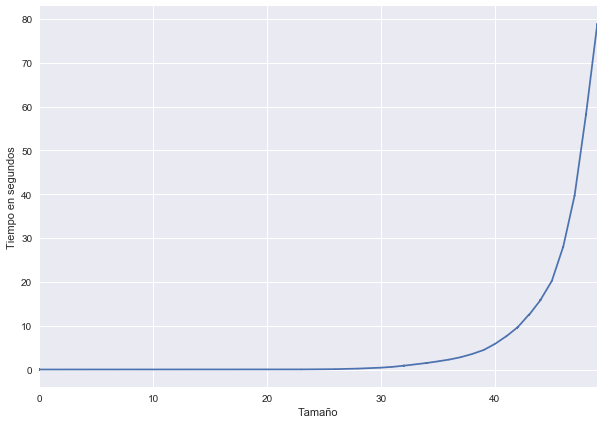
\includegraphics[width=.8\textwidth]{ej1.png}
	\end{center}

\pagebreak
\section{Mejora del algoritmo propuesto (poda de resultados)}
	\subsection{Descripción del algorítmo}

	Las podas apuntan a obviar el cálculo de soluciones que ya sabemos peores que otras ya calculadas:

	\begin{itemize}

		\item Si sabemos que en alguna rama encontramos una solución final de tamaño i y la rama actual tiene una solución parcial de $j \leq i$, podemos obviar el resto de la rama actual.

		\item Si sabemos que existe una rama con solución final 0, existe una solución óptima y no requerimos calcular nada más.

	\end{itemize}

	A continuación se propone un algoritmo para las llamadas recursivas. Para el caso inicial, se toma $Indice = 0$, $Actual = 0$ y $Mejor = |Lista|$.

	La variable $Mejor$ es de entrada/salida, es decir, las llamadas recursivas pueden modificar el valor. Al final del algoritmo, la misma almacenará el mejor resultado.

	\begin{algorithm}[H]
		\NoCaptionOfAlgo
		
		\KwData{Lista, la lista de números a pintar}

		\KwData{UltRojo, el valor del úlitmo rojo que pintamos}

		\KwData{UltAzul, el valor del úlitmo azul que pintamos}

		\KwData{Indice, la posición que estamos mirando ahora}

		\KwData{Actual, la cantidad de elemntos no pintados hasta ahora}

		\KwData{Mejor, la mejor solución hasta ahora}

		\If{Actual $<$ Mejor} {
			\uIf{Indice == $|Lista|$}{
				Llegamos al final de la lista

				Mejor es Actual
			}
			\Else{
				\If{no existe UltRojo \textbf{or} UltRojo $<$ Lista[Indice]}{
					Calcular el mejor resultado pintando de Rojo

					Llamada Recursiva: \{Lista, Lista[Indice], UltAzul, Indice+1, Res, Mejor\}

					La función modifica el valor de Mejor si corresponde
				}
				\If{Mejor $\neq$ 0}{
					\If{no existe UltAzul \textbf{or} UltAzul $>$ Lista[Indice]}{
						Calcular el mejor resultado pintando de Azul

						Llamada Recursiva: \{Lista, UltRojo, Lista[Indice], Indice+1, Res, Mejor\}

						La función modifica el valor de Mejor si corresponde
					}
					\If{Mejor $\neq$ 0}{
						Calcular el mejor resultado sin pintar

						Llamada Recursiva: \{Lista, UltRojo, UltAzul, Indice+1, Res+1, Mejor\}

						La función modifica el valor de Mejor si corresponde
					}
				}
			}
		}

		\KwResult{Ninguno, pero Mejor puede ser modificado si se encuentra una mejor subsolución.}
	\end{algorithm}

	A diferencia del algoritmo de Backtracking básico, el orden en que se calculan los casos recursivos es importante, ya que podemos encontrar un caso óptimo y podar el resto del espacio de soluciones.

	\pagebreak
	\subsection{Cota de complejidad}

	El algoritmo propuesto, al igual que el algorítmo base de Backtracking, realiza hasta tres llamadas recursivas en cada paso. En mejor caso, no se realiza ninguna llamada recursiva (se realiza una poda).

	En cualquier llamada recursiva, el tamaño del problema a resolver disminuye en 1 (se avanza/pinta un solo número).

	La función de complejidad sería
	\[
	T(BTMejorado(n)) =
		\begin{cases}
			\text{1,} &\quad\text{si n == 0}\\
			\text{3 T(BTMejorado(n-1)),} &\quad\text{si no} \\
		\end{cases}
	\]

	donde n es la cantidad de números restantes, es decir, $|Lista| - Indice$.

	Es decir, en órdenes de complejidad, BTMejorado (Backtracking con podas) es igual a BT (Backtracking sin podas).

	Esto no quiere decir que las podas son irrelevantes, las mismas pueden cortar el tiempo de procesamiento de manera importante, pero los cambios en complejidad son de orden menor a $3^n$, por lo que esta sigue siendo la complejidad en peor caso.

	El mejor caso para el algoritmo se da si la lista es estrictamente creciente. En este caso, se realiza solo una llamada recursiva por nivel, hallando un caso óptimo al llegar al final de la lista y podando el resto, por lo que la complejidad resultante es de $\Omega(n)$.

	Este es un detalle implementativo, ya que en el algoritmo propuesto primero se realizan las llamdadas recursivas pintando de rojo de ser posible. De haberse utilizado un orden distinto, el mejor caso podría haberse dado con una entrada diferente.

	\subsection{Gráfico de complejidad}

	El siguiente gráfico utiliza el mismo criterio que el anterior. Si bien la diferencia no es visualmente notoria, debe notarse que los valores del eje vertical son mucho menores (alrededor de 1/10 de los valores equivalentes sin poda).

	\begin{center}
	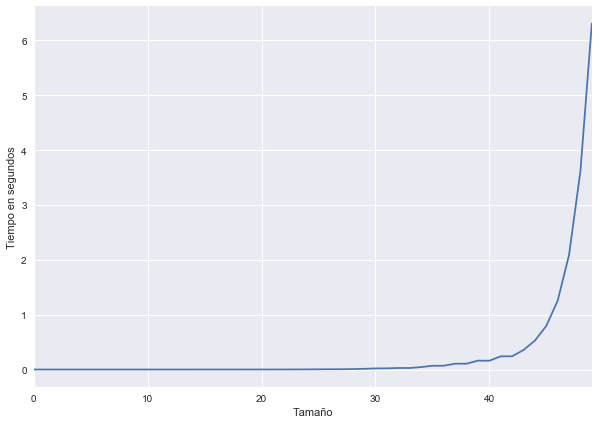
\includegraphics[width=.8\textwidth]{ej2.png}
	\end{center}

	Se agrega también el siguiente gráfico en el que se muestran ambos algoritmos, utilizando una escala logarítmica para poder comparar mejor los órdenes de complejidad. El algoritmo mejorado es irregular debido a que las listas testeadas son aleatorias y pueden tener mejor o peor comportamiento frente a las podas definidas.

	Como evidencia el gráfico logarítmico, si bien la mejora con las podas es notoria (como se mencionó antes, aproximadamente 1/10 del tiempo), ambos algorítmos crecen en órdenes similares.

	\begin{center}
	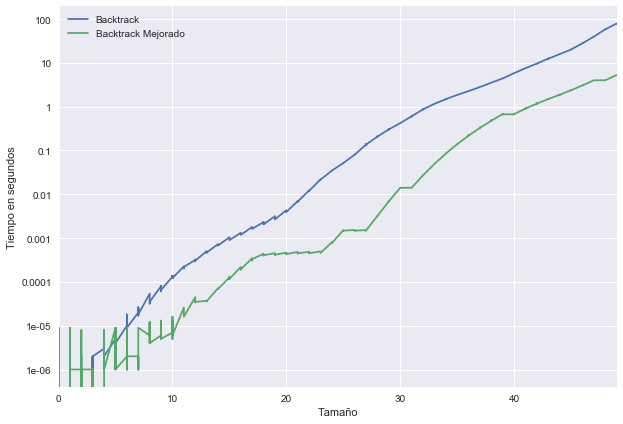
\includegraphics[width=.8\textwidth]{ej2-2.png}
	\end{center}

	Como nota final, al analizar el mejor caso del algoritmo, el tiempo de procesado de estas era casi despreciable ya que la complejidad es lineal al tamaño de la lista. Por este motivo, no es práctico comparar estos casos, pero si se incluye un gráfico ilustrativo de dicho caso, medido con listas de enteros consecutivos entre 1 y $|Lista|$. Notese que el tiempo está medido en nanosegundos por el requerimiento de precisión extrema, y las mediciones tienen ruido por procesamiento ajeno al problema.

	\begin{center}
	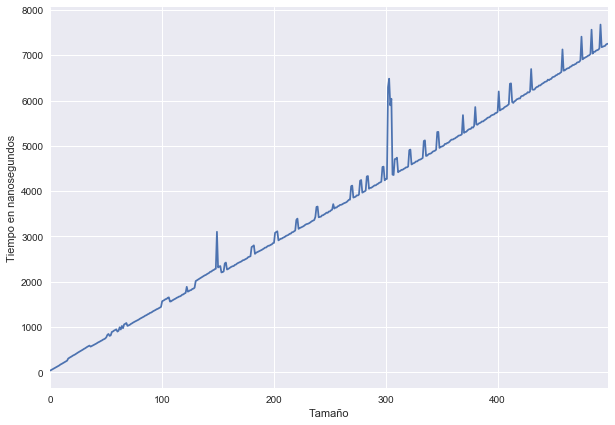
\includegraphics[width=.8\textwidth]{ej2-3.png}
	\end{center}

\pagebreak
\section{Resolución por \textit{Programación Dinámica}}
	\subsection{Descripción del algorítmo}

	La solución por Programación Dinámica utiliza memoización: casos menores se guardan en una memoria interna y son reutilizados para calcular casos mayores.

	En el algoritmo que se propone, la memoria toma forma de arreglo de dos dimensiones, donde cada dimensión expresa la posición en la lista donde se encuentra el último elemento pintado de uno u otro color. Al calcular un casillero, se toma el color más avanzado y se recorren los anteriores para encontrar la mejor subsolución.

	Se debe considerar que no se calcula ninguno de los valores correspondientes a la diagonal de este arreglo, es decir, posiciones que representarían que un mismo elemento está pintado de ambos colores, ya que esto no es válido.

	\begin{algorithm}[H]
		\NoCaptionOfAlgo
		
		\KwData{Lista, la lista de números a pintar}

		\KwData{Memoria, el arreglo de dos dimensiones con soluciones previas}

		\KwData{Rojo, la posición del rojo que estamos calculando ahora}

		\KwData{Azul, la posición del azul que estamos calculando ahora}

		\If{Memoria[Rojo][Azul] no fue calculado todavía}{
			\uIf{Rojo == Azul == $|Lista|$}{
				Estamos en el caso base (nada pintado)

				Guardamos en Memoria[Rojo][Azul] |Lista| (todos sin pintar) y lo marcamos como calculado
			}
			\uElseIf{Azul == |$Lista|$ \textbf{or} Rojo $>$ Azul}{
				Buscamos el mejor valor para los rojos anteriores.

				\For{i $\leftarrow$ 0 \KwTo Rojo - 1}{
					\If{i $\neq$ Azul}{
						Llamada recursiva: \{Lista, Memoria, i, Azul\}
					}
				}

				Llamadas recursiva: \{Lista, Memoria, $|Lista|$, Azul\} (caso sin pintar rojos)

				Sea Min el menor resultado de todas las llamadas recursivas

				Guardamos en Memoria[Rojo][Azul] Min - 1 (fue pintado Rojo) y lo marcamos como calculado
			}
			\Else{
				Buscamos el mejor valor para los azules anteriores.

				\For{i $\leftarrow$ 0 \KwTo Azul - 1}{
					\If{i $\neq$ Rojo}{
						Llamada recursiva: \{Lista, Memoria, Rojo, i\}
					}
				}

				Llamada recursiva: \{Lista, Memoria, Rojo, $|Lista|$\} (caso sin pintar azules)

				Sea Min el menor resultado de todas las llamadas recursivas

				Guardamos en Memoria[Rojo][Azul] Min - 1 (fue pintado Azul) y lo marcamos como calculado
			}
		}

		\KwResult{Memoria[Rojo][Azul]}
	\end{algorithm}

	En la implementación provista, la memoria se rellena de forma \textit{bottom-up}, es decir los casos más básicos primero, pero el orden no altera el producto ya que en cada paso la llamada recursiva asegura que cualquier posición que se necesite esté calculada, y solo se calcula una vez.

	A su vez, cada dimensión de la memoria tiene de un casillero de largo extra para considerar el caso en que no se han pintado todavía casilleros de ese color. La memoria almacena si ya fue calculada y el mejor resultado posible para la misma.

	\subsection{Cota de complejidad}

	Este algoritmo realiza, en peor caso, n llamadas recursivas por paso. Sin embargo, como cada resultado se memoiza, cada llamada recursiva cuesta O(1) amortizado.

	Como el algoritmo rellena toda la memoria (salvo las posiciones inválidas), y el tamaño de la misma es de $n^2$ (siendo n el largo de la lista), el orden de complejidad del algoritmo es $O(n^3)$.

	\pagebreak
	\subsection{Gráfico de complejidad}

	El siguiente gráfico, si bien fue medido de la misma manera que los otros, utiliza una escala en microsegundos. Tanto la forma de la figura, más gradual que en los gráficos anteriores, como la necesidad de usar una unidad de medida más precisa dejan en claro que este algoritmo es mucho más eficiente.

	\begin{center}
	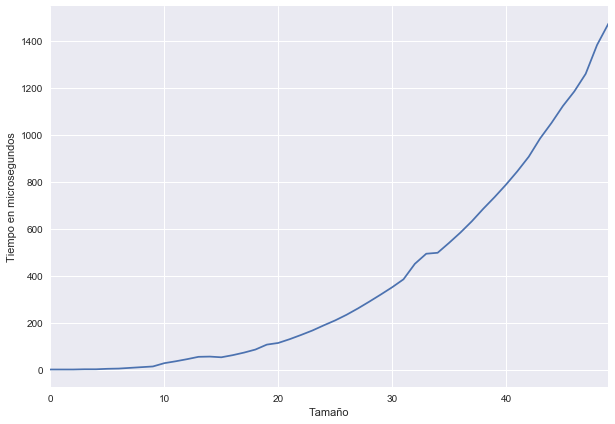
\includegraphics[width=.8\textwidth]{ej3.png}
	\end{center}

	A modo de comparación se agrega también el siguiente gráfico en el que se muestran los tres algoritmos utilizando la escala logarítmica, y utilizando nuevamente segundos para el eje Y.

	En este caso se puede notar la diferencia en orden de complejidad comparado con los algoritmos basados en Backtracking: mientras que aquellos se asemejan levemente a una recta lineal en escala logarítmica (por su complejidad exponencial), este algoritmo es polinómico y por ende describe una curva logarítmica.

	\begin{center}
	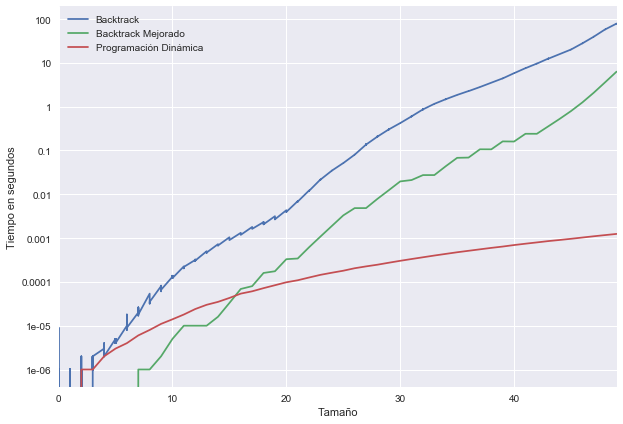
\includegraphics[width=.8\textwidth]{ej3-2.png}
	\end{center}

\pagebreak
\section{Apéndices}
	\subsection{Apéndice I: generación de datos}
	Para poder analizar las complejidades de los algoritmos propuestos, se utilizaron las siguientes herramientas para generar mediciones y graficar datos:

	\begin{itemize}
		\item Un generador de listas aleatorias basadas en \texttt{std::rand()} (parte de la biblioteca estándar de C++).

		\begin{algorithm}[H]
		\NoCaptionOfAlgo

		\For{i $\leftarrow$ 0 \KwTo n - 1}{
			Lista[i] $\leftarrow$ std::rand()
		}
		\end{algorithm}

		Cada una de estas listas se guardo en una memoria temporal para poder probar los tres algoritmos con el mismo input.

		\item Un generador de listas secuenciales para el mejor caso de Backtracking con podas

		\begin{algorithm}[H]
		\NoCaptionOfAlgo
		

		\For{i $\leftarrow$ 0 \KwTo n - 1}{
			Lista[i] $\leftarrow$ i()
		}
		\end{algorithm}

		Este generador se usa en partiuclar para el ejercicio 2. Si bien las entradas fueron probadas en otros algoritmos, solo el Backtracking con podas puede sacar mayor provecho de esta entrada, y tiene un impacto relevante y fácil de medir en su performance.

		\item Mediciones de tiempo con \texttt{std::chrono} (parte de la biblioteca estándar de C++11).

		\begin{algorithm}[H]
		\NoCaptionOfAlgo

		Sea Mejor el mejor tiempo medido (todavía no inicializado)
		\For{i $\leftarrow$ 0 \KwTo Repeticiones - 1}{
			Comienzo $\leftarrow$ \texttt{std::chrono::high\_resolution\_clock::now()}

			Invocar Resolver(lista) (correspondiente al algoritmo)

			Fin $\leftarrow$ \texttt{std::chrono::high\_resolution\_clock::now()}

			Actual $\leftarrow$ \texttt{std::chrono::duration\_cast<std::chrono::microseconds>(Fin - Comienzo).count()}

			\If{Mejor no está inicializado \textbf{or} Actual $<$ Mejor}{

				Mejor $\leftarrow$ Actual
			}
		}
		\end{algorithm}

		Cada algoritmo fue probado varias veces con cada entrada, conservando solo el valor de tiempo menor para reducir el ruido por procesos ajenos al problema.

		La unidad de medición preferida fue microsegundos (\texttt{std::chrono::microseconds}, $seg \times 10^{-6}$), pero también se utilizó nanosegundos en algunas ocasiones, y los gráficos fueron escalados a segundos cuando correspondía por la dimensión de las variables.

		\item Graficado con \texttt{matplotlib.pyplot} y \texttt{pandas} (con Python y Jupyter Notebook)

		Se utilizaron los DataFrames de Pandas para el manejo de datos (guardados en \texttt{.csv}) y el graficado, en conjunto con matplotlib. Por el escalado a segundos, algunos detalles de los ejes se manejaron a mano con matplotlib.

	\end{itemize}

	\subsection{Apéndice II: herramientas de compilación y testing}
	Durante el desarrollo se utilizaron las siguientes herramientas:

	\begin{itemize}
		\item CMake

		Se decidió utilizar CMake para la compilación por su simplicidad y compatibilidad con otras herramientras. Junto con el código se provee el archivo \texttt{CMakeLists.txt} para compilar el mismo.

		\item Google Test

		Para generar tests unitarios con datos reutilizables se usó Google Test. Dichos archivos eran importados por otro \texttt{CMakeLists.txt} y no están incluídos en la presente entrega del trabajo práctico.

		\item Namespace \texttt{Utils}

		Dentro de \texttt{Utils.h} se definieron 2 funciones útiles para el trabajo práctico: una de ellas crea un vector desde el stdin, para ser usado en los tres ejercicios; la otra es una función de logging que fue utilizada al programar para detectar errores y ver otros detalles del proceso.

		La función \texttt{log} sigue estando incluída en los algoritmos, pero su funcionalidad se encuentra apagada por un \texttt{\#define} y no debería generar ningún costo adicional (ya que usa printf por detrás y no genera el output salvo que sea necesario).
	\end{itemize}


\end{document}